\section{PToPSwitchArbiter Class Reference}
\label{classPToPSwitchArbiter}\index{PToPSwitchArbiter@{PToPSwitchArbiter}}
{\tt \#include $<$ptop\_\-swa.h$>$}

Collaboration diagram for PToPSwitchArbiter:\nopagebreak
\begin{figure}[H]
\begin{center}
\leavevmode
\includegraphics[width=400pt]{classPToPSwitchArbiter__coll__graph}
\end{center}
\end{figure}
\subsection*{Public Member Functions}
\begin{CompactItemize}
\item 
{\bf PToPSwitchArbiter} ()
\item 
{\bf $\sim$PToPSwitchArbiter} ()
\item 
void {\bf resize} ({\bf uint} p)
\item 
bool {\bf is\_\-requested} ({\bf uint} outp, {\bf uint} inp)
\item 
void {\bf request} ({\bf uint} p, {\bf uint} inp)
\item 
{\bf SA\_\-unit} {\bf pick\_\-winner} ({\bf uint} p)
\item 
{\bf SA\_\-unit} {\bf do\_\-round\_\-robin\_\-arbitration} ({\bf uint} p)
\item 
{\bf SA\_\-unit} {\bf do\_\-priority\_\-round\_\-robin\_\-arbitration} ({\bf uint} p)
\item 
{\bf SA\_\-unit} {\bf do\_\-fcfs\_\-arbitration} ({\bf uint} p)
\item 
void {\bf clear\_\-winner} ({\bf uint} p, {\bf uint} ip)
\item 
void {\bf clear\_\-requested} ({\bf uint} p, {\bf uint} ip)
\item 
void {\bf request} ({\bf uint} oport, {\bf uint} inport, {\bf message\_\-class} m)
\item 
bool {\bf is\_\-empty} ()
\item 
string {\bf toString} () const 
\end{CompactItemize}
\subsection*{Public Attributes}
\begin{CompactItemize}
\item 
{\bf uint} {\bf address}
\item 
string {\bf name}
\item 
{\bf uint} {\bf node\_\-ip}
\end{CompactItemize}
\subsection*{Private Attributes}
\begin{CompactItemize}
\item 
{\bf uint} {\bf PORTS}
\item 
{\bf uint} {\bf CHANNELS}
\item 
vector$<$ bool $>$ {\bf locked}
\item 
vector$<$ bool $>$ {\bf done}
\item 
vector$<$ vector$<$ bool $>$ $>$ {\bf requested}
\item 
vector$<$ vector$<$ bool $>$ $>$ {\bf priority\_\-reqs}
\item 
vector$<$ bool $>$ {\bf port\_\-locked}
\item 
vector$<$ vector$<$ {\bf SA\_\-unit} $>$ $>$ {\bf requesting\_\-inputs}
\item 
vector$<$ {\bf SA\_\-unit} $>$ {\bf last\_\-winner}
\item 
vector$<$ {\bf uint} $>$ {\bf last\_\-port\_\-winner}
\end{CompactItemize}


\subsection{Detailed Description}


Definition at line 30 of file ptop\_\-swa.h.

\subsection{Constructor \& Destructor Documentation}
\index{PToPSwitchArbiter@{PToPSwitchArbiter}!PToPSwitchArbiter@{PToPSwitchArbiter}}
\index{PToPSwitchArbiter@{PToPSwitchArbiter}!PToPSwitchArbiter@{PToPSwitchArbiter}}
\subsubsection[{PToPSwitchArbiter}]{\setlength{\rightskip}{0pt plus 5cm}PToPSwitchArbiter::PToPSwitchArbiter ()}\label{classPToPSwitchArbiter_dc9c6f383f3f135ca2fa003380b52021}




Definition at line 24 of file ptop\_\-swa.cc.

References name.\index{PToPSwitchArbiter@{PToPSwitchArbiter}!$\sim$PToPSwitchArbiter@{$\sim$PToPSwitchArbiter}}
\index{$\sim$PToPSwitchArbiter@{$\sim$PToPSwitchArbiter}!PToPSwitchArbiter@{PToPSwitchArbiter}}
\subsubsection[{$\sim$PToPSwitchArbiter}]{\setlength{\rightskip}{0pt plus 5cm}PToPSwitchArbiter::$\sim$PToPSwitchArbiter ()}\label{classPToPSwitchArbiter_f59e4ed8cfb944b1ca266cdfc413b078}




Definition at line 29 of file ptop\_\-swa.cc.

\subsection{Member Function Documentation}
\index{PToPSwitchArbiter@{PToPSwitchArbiter}!clear\_\-requested@{clear\_\-requested}}
\index{clear\_\-requested@{clear\_\-requested}!PToPSwitchArbiter@{PToPSwitchArbiter}}
\subsubsection[{clear\_\-requested}]{\setlength{\rightskip}{0pt plus 5cm}void PToPSwitchArbiter::clear\_\-requested ({\bf uint} {\em p}, \/  {\bf uint} {\em ip})}\label{classPToPSwitchArbiter_c21620597bbc0344eec88c21b254a310}




Definition at line 299 of file ptop\_\-swa.cc.

References priority\_\-reqs, and requested.

Referenced by GenericRouterVct::do\_\-switch\_\-allocation(), and GenericRouterAdaptive::do\_\-switch\_\-allocation().

Here is the caller graph for this function:\nopagebreak
\begin{figure}[H]
\begin{center}
\leavevmode
\includegraphics[width=420pt]{classPToPSwitchArbiter_c21620597bbc0344eec88c21b254a310_icgraph}
\end{center}
\end{figure}
\index{PToPSwitchArbiter@{PToPSwitchArbiter}!clear\_\-winner@{clear\_\-winner}}
\index{clear\_\-winner@{clear\_\-winner}!PToPSwitchArbiter@{PToPSwitchArbiter}}
\subsubsection[{clear\_\-winner}]{\setlength{\rightskip}{0pt plus 5cm}void PToPSwitchArbiter::clear\_\-winner ({\bf uint} {\em p}, \/  {\bf uint} {\em ip})}\label{classPToPSwitchArbiter_752c022c63e6552d06798d65e634f8d4}




Definition at line 288 of file ptop\_\-swa.cc.

References done, locked, priority\_\-reqs, and requested.

Referenced by GenericRouterVct::do\_\-switch\_\-traversal(), GenericRouterNoVcs::do\_\-switch\_\-traversal(), and GenericRouterAdaptive::do\_\-switch\_\-traversal().

Here is the caller graph for this function:\nopagebreak
\begin{figure}[H]
\begin{center}
\leavevmode
\includegraphics[width=420pt]{classPToPSwitchArbiter_752c022c63e6552d06798d65e634f8d4_icgraph}
\end{center}
\end{figure}
\index{PToPSwitchArbiter@{PToPSwitchArbiter}!do\_\-fcfs\_\-arbitration@{do\_\-fcfs\_\-arbitration}}
\index{do\_\-fcfs\_\-arbitration@{do\_\-fcfs\_\-arbitration}!PToPSwitchArbiter@{PToPSwitchArbiter}}
\subsubsection[{do\_\-fcfs\_\-arbitration}]{\setlength{\rightskip}{0pt plus 5cm}{\bf SA\_\-unit} PToPSwitchArbiter::do\_\-fcfs\_\-arbitration ({\bf uint} {\em p})}\label{classPToPSwitchArbiter_3e59f4eb3486f1b5355476c50550f702}




Definition at line 244 of file ptop\_\-swa.cc.

References \_\-DBG\_\-NOARG, done, last\_\-winner, locked, Simulator::Now(), PORTS, requested, and requesting\_\-inputs.

Referenced by pick\_\-winner().

Here is the caller graph for this function:\nopagebreak
\begin{figure}[H]
\begin{center}
\leavevmode
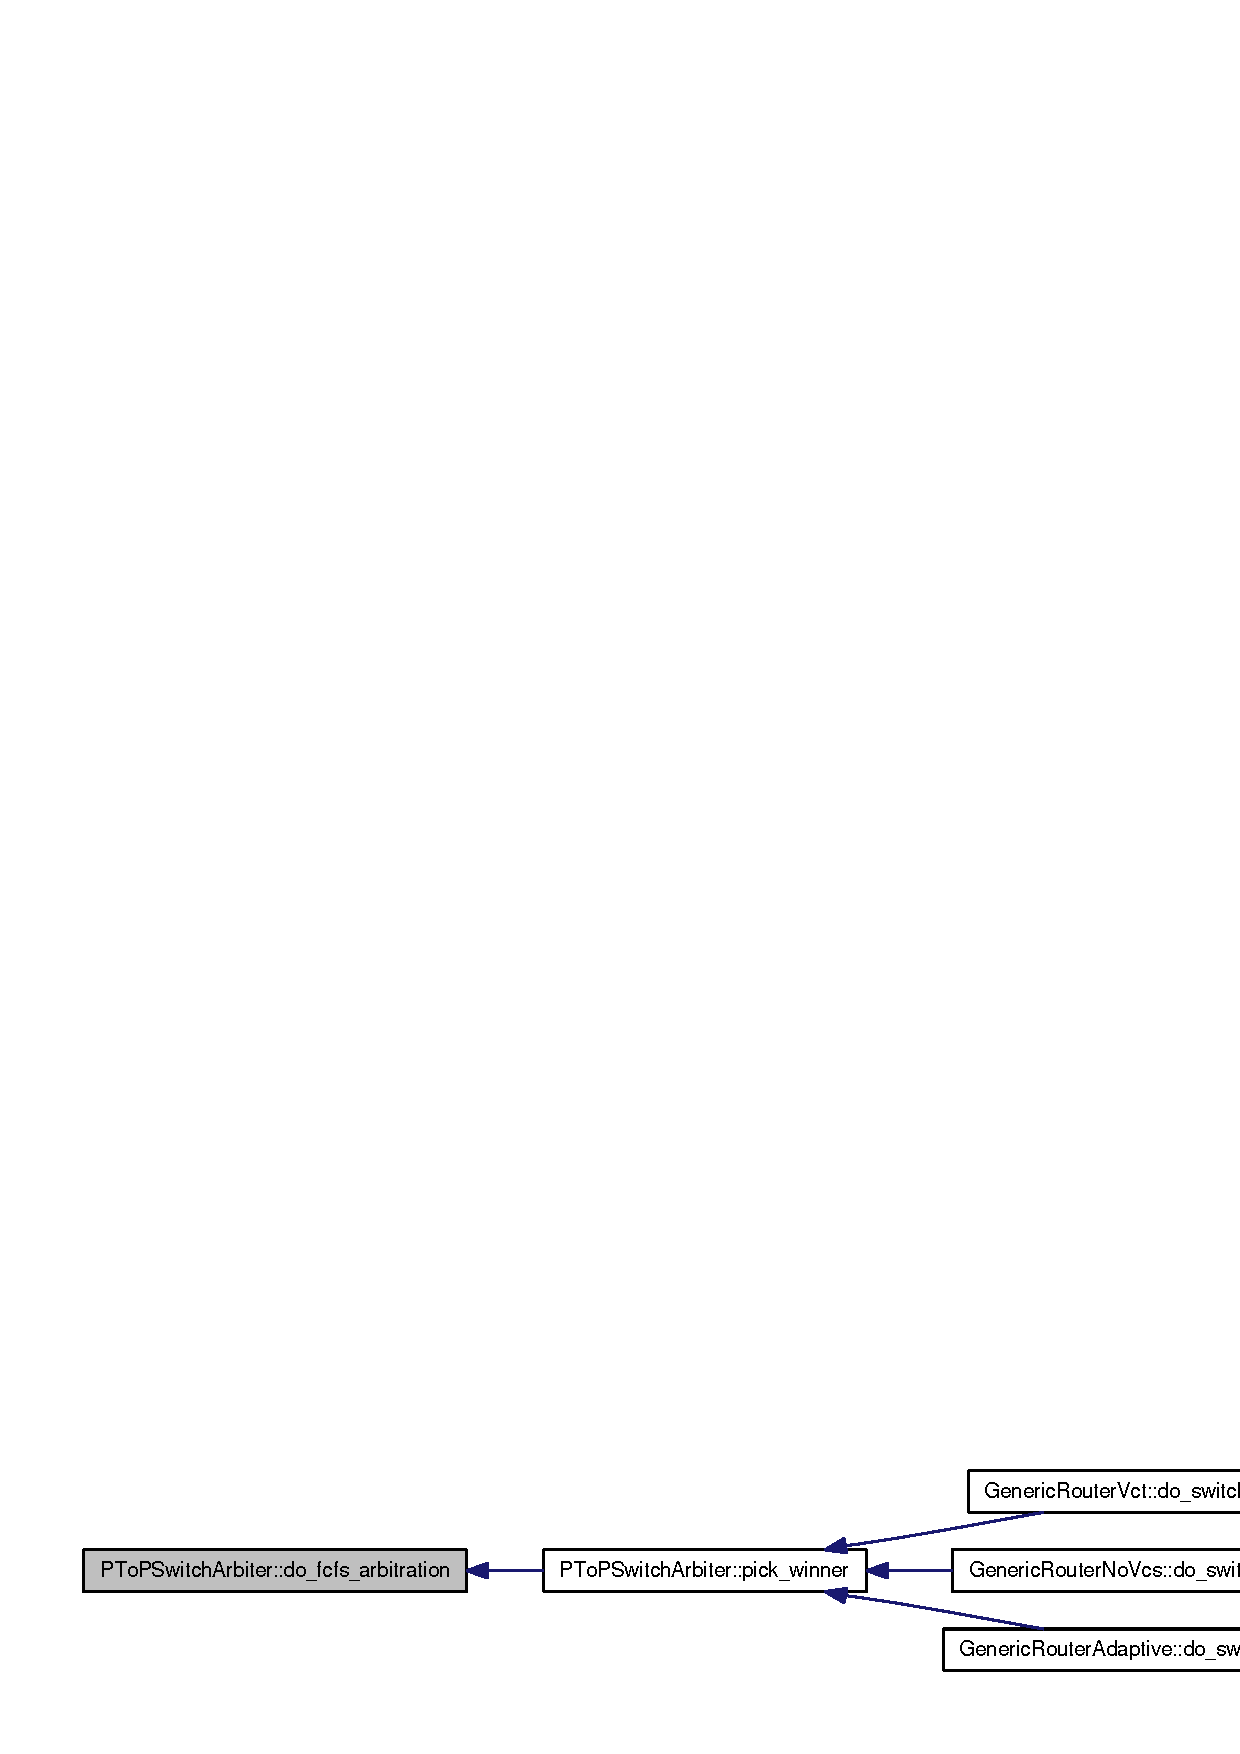
\includegraphics[width=420pt]{classPToPSwitchArbiter_3e59f4eb3486f1b5355476c50550f702_icgraph}
\end{center}
\end{figure}
\index{PToPSwitchArbiter@{PToPSwitchArbiter}!do\_\-priority\_\-round\_\-robin\_\-arbitration@{do\_\-priority\_\-round\_\-robin\_\-arbitration}}
\index{do\_\-priority\_\-round\_\-robin\_\-arbitration@{do\_\-priority\_\-round\_\-robin\_\-arbitration}!PToPSwitchArbiter@{PToPSwitchArbiter}}
\subsubsection[{do\_\-priority\_\-round\_\-robin\_\-arbitration}]{\setlength{\rightskip}{0pt plus 5cm}{\bf SA\_\-unit} PToPSwitchArbiter::do\_\-priority\_\-round\_\-robin\_\-arbitration ({\bf uint} {\em p})}\label{classPToPSwitchArbiter_012ef93786c879ce0c3db3891d43a9be}




Definition at line 176 of file ptop\_\-swa.cc.

References \_\-DBG\_\-NOARG, done, last\_\-port\_\-winner, last\_\-winner, locked, PORTS, priority\_\-reqs, requested, and requesting\_\-inputs.

Referenced by pick\_\-winner().

Here is the caller graph for this function:\nopagebreak
\begin{figure}[H]
\begin{center}
\leavevmode
\includegraphics[width=420pt]{classPToPSwitchArbiter_012ef93786c879ce0c3db3891d43a9be_icgraph}
\end{center}
\end{figure}
\index{PToPSwitchArbiter@{PToPSwitchArbiter}!do\_\-round\_\-robin\_\-arbitration@{do\_\-round\_\-robin\_\-arbitration}}
\index{do\_\-round\_\-robin\_\-arbitration@{do\_\-round\_\-robin\_\-arbitration}!PToPSwitchArbiter@{PToPSwitchArbiter}}
\subsubsection[{do\_\-round\_\-robin\_\-arbitration}]{\setlength{\rightskip}{0pt plus 5cm}{\bf SA\_\-unit} PToPSwitchArbiter::do\_\-round\_\-robin\_\-arbitration ({\bf uint} {\em p})}\label{classPToPSwitchArbiter_bb10205ca5104e0be5519bd336fb85e1}




Definition at line 120 of file ptop\_\-swa.cc.

References \_\-DBG\_\-NOARG, done, last\_\-port\_\-winner, last\_\-winner, locked, PORTS, requested, and requesting\_\-inputs.

Referenced by pick\_\-winner().

Here is the caller graph for this function:\nopagebreak
\begin{figure}[H]
\begin{center}
\leavevmode
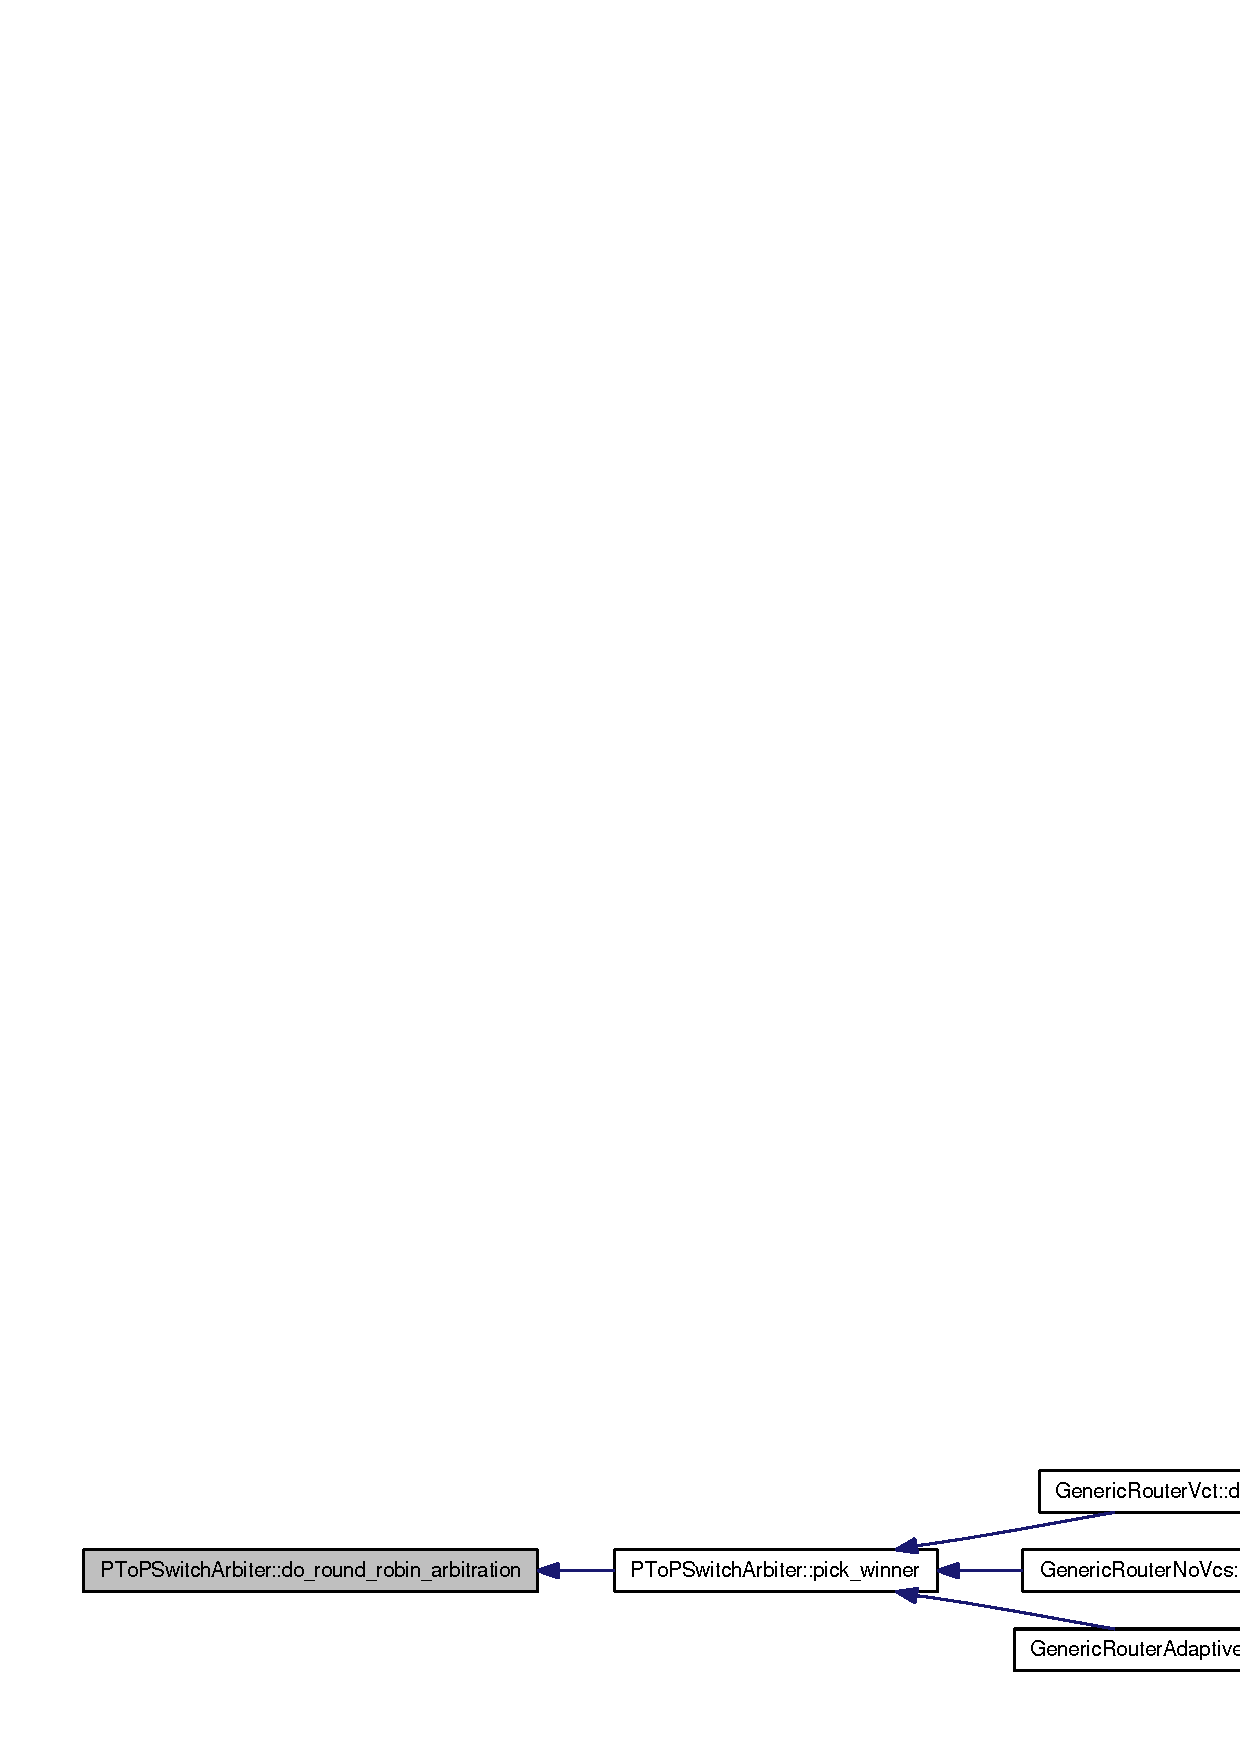
\includegraphics[width=420pt]{classPToPSwitchArbiter_bb10205ca5104e0be5519bd336fb85e1_icgraph}
\end{center}
\end{figure}
\index{PToPSwitchArbiter@{PToPSwitchArbiter}!is\_\-empty@{is\_\-empty}}
\index{is\_\-empty@{is\_\-empty}!PToPSwitchArbiter@{PToPSwitchArbiter}}
\subsubsection[{is\_\-empty}]{\setlength{\rightskip}{0pt plus 5cm}bool PToPSwitchArbiter::is\_\-empty (void)}\label{classPToPSwitchArbiter_20a229615b20e987aaa0291af0805e31}




Definition at line 307 of file ptop\_\-swa.cc.

References PORTS, and requested.

Referenced by GenericRouterVct::do\_\-switch\_\-allocation(), GenericRouterNoVcs::do\_\-switch\_\-allocation(), and GenericRouterAdaptive::do\_\-switch\_\-allocation().

Here is the caller graph for this function:\nopagebreak
\begin{figure}[H]
\begin{center}
\leavevmode
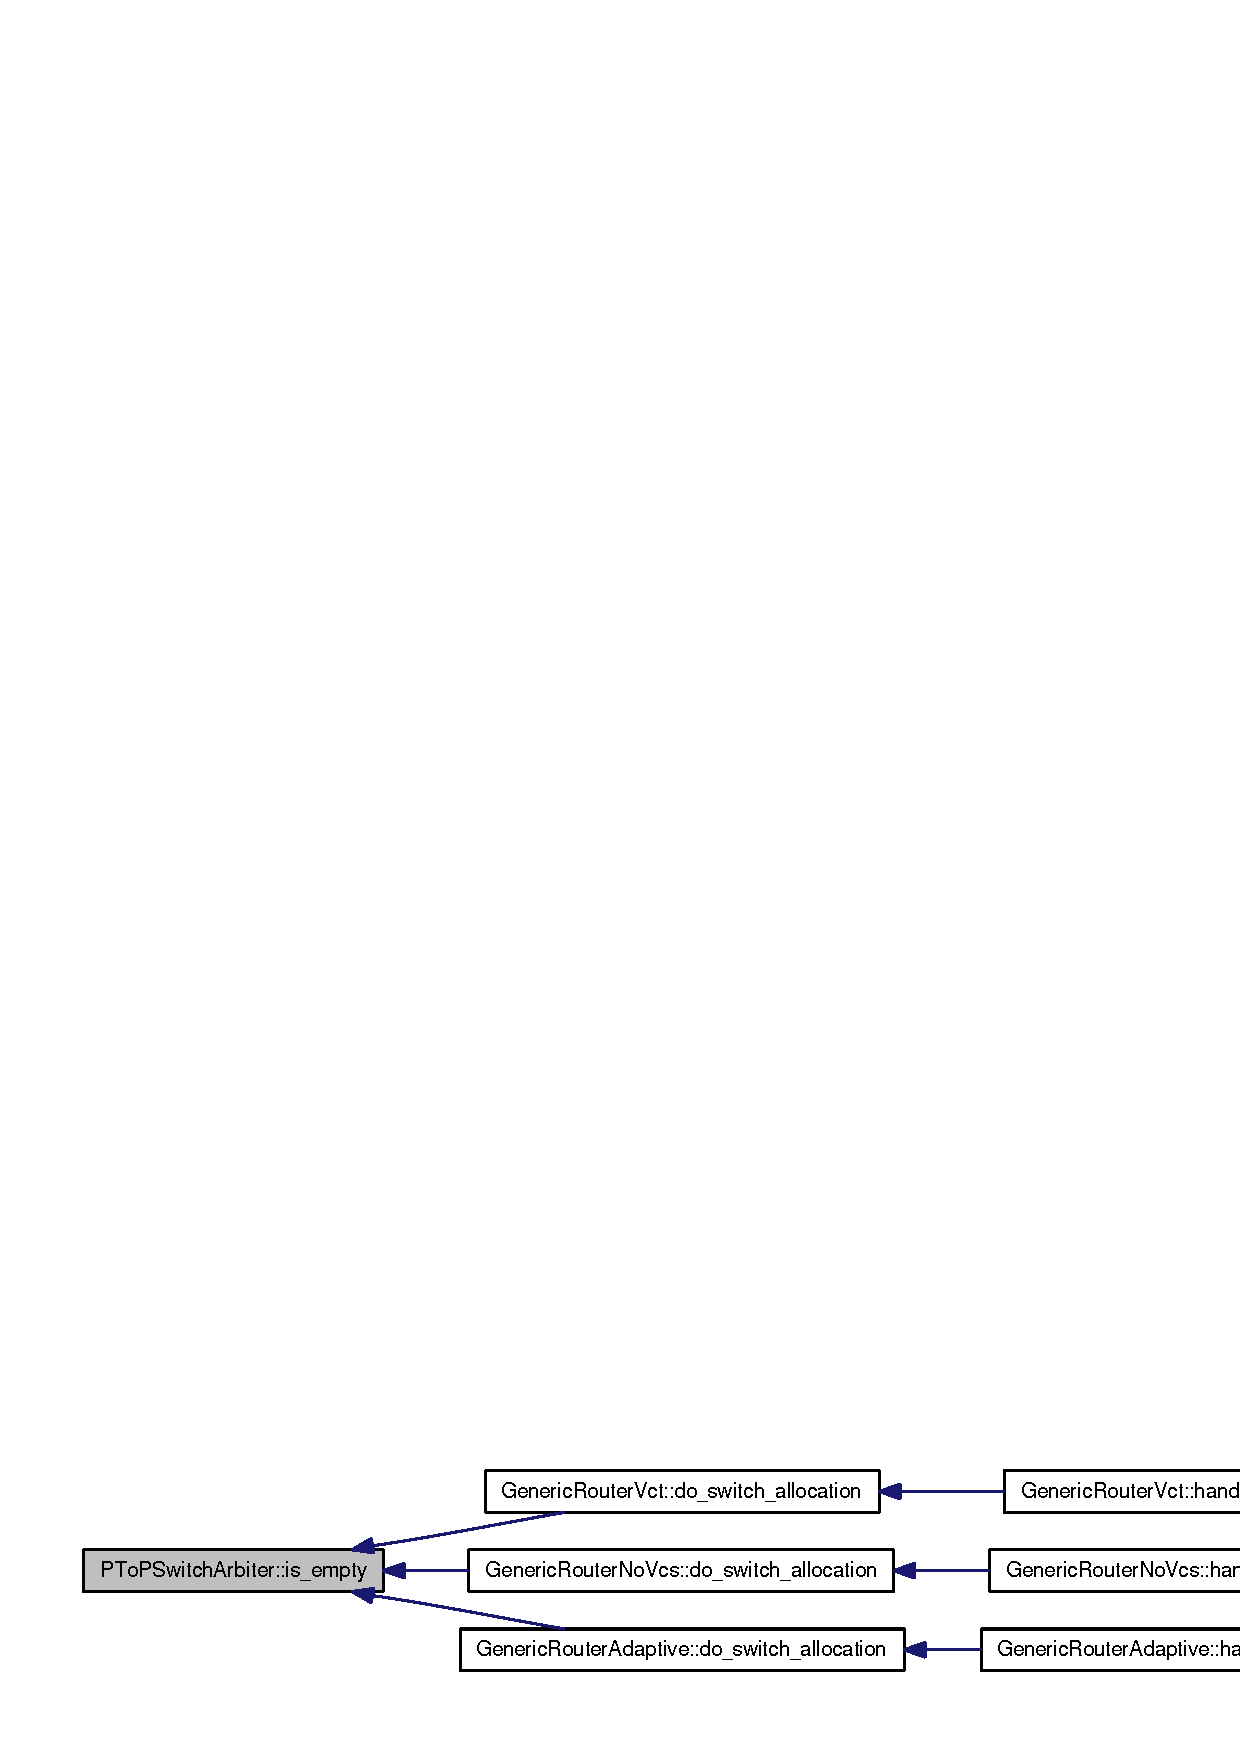
\includegraphics[width=420pt]{classPToPSwitchArbiter_20a229615b20e987aaa0291af0805e31_icgraph}
\end{center}
\end{figure}
\index{PToPSwitchArbiter@{PToPSwitchArbiter}!is\_\-requested@{is\_\-requested}}
\index{is\_\-requested@{is\_\-requested}!PToPSwitchArbiter@{PToPSwitchArbiter}}
\subsubsection[{is\_\-requested}]{\setlength{\rightskip}{0pt plus 5cm}bool PToPSwitchArbiter::is\_\-requested ({\bf uint} {\em outp}, \/  {\bf uint} {\em inp})}\label{classPToPSwitchArbiter_3c4eeb723ecb521a82a4518820e48896}




Definition at line 69 of file ptop\_\-swa.cc.

References requested.

Referenced by GenericRouterVct::handle\_\-tick\_\-event(), GenericRouterNoVcs::handle\_\-tick\_\-event(), and GenericRouterAdaptive::handle\_\-tick\_\-event().

Here is the caller graph for this function:\nopagebreak
\begin{figure}[H]
\begin{center}
\leavevmode
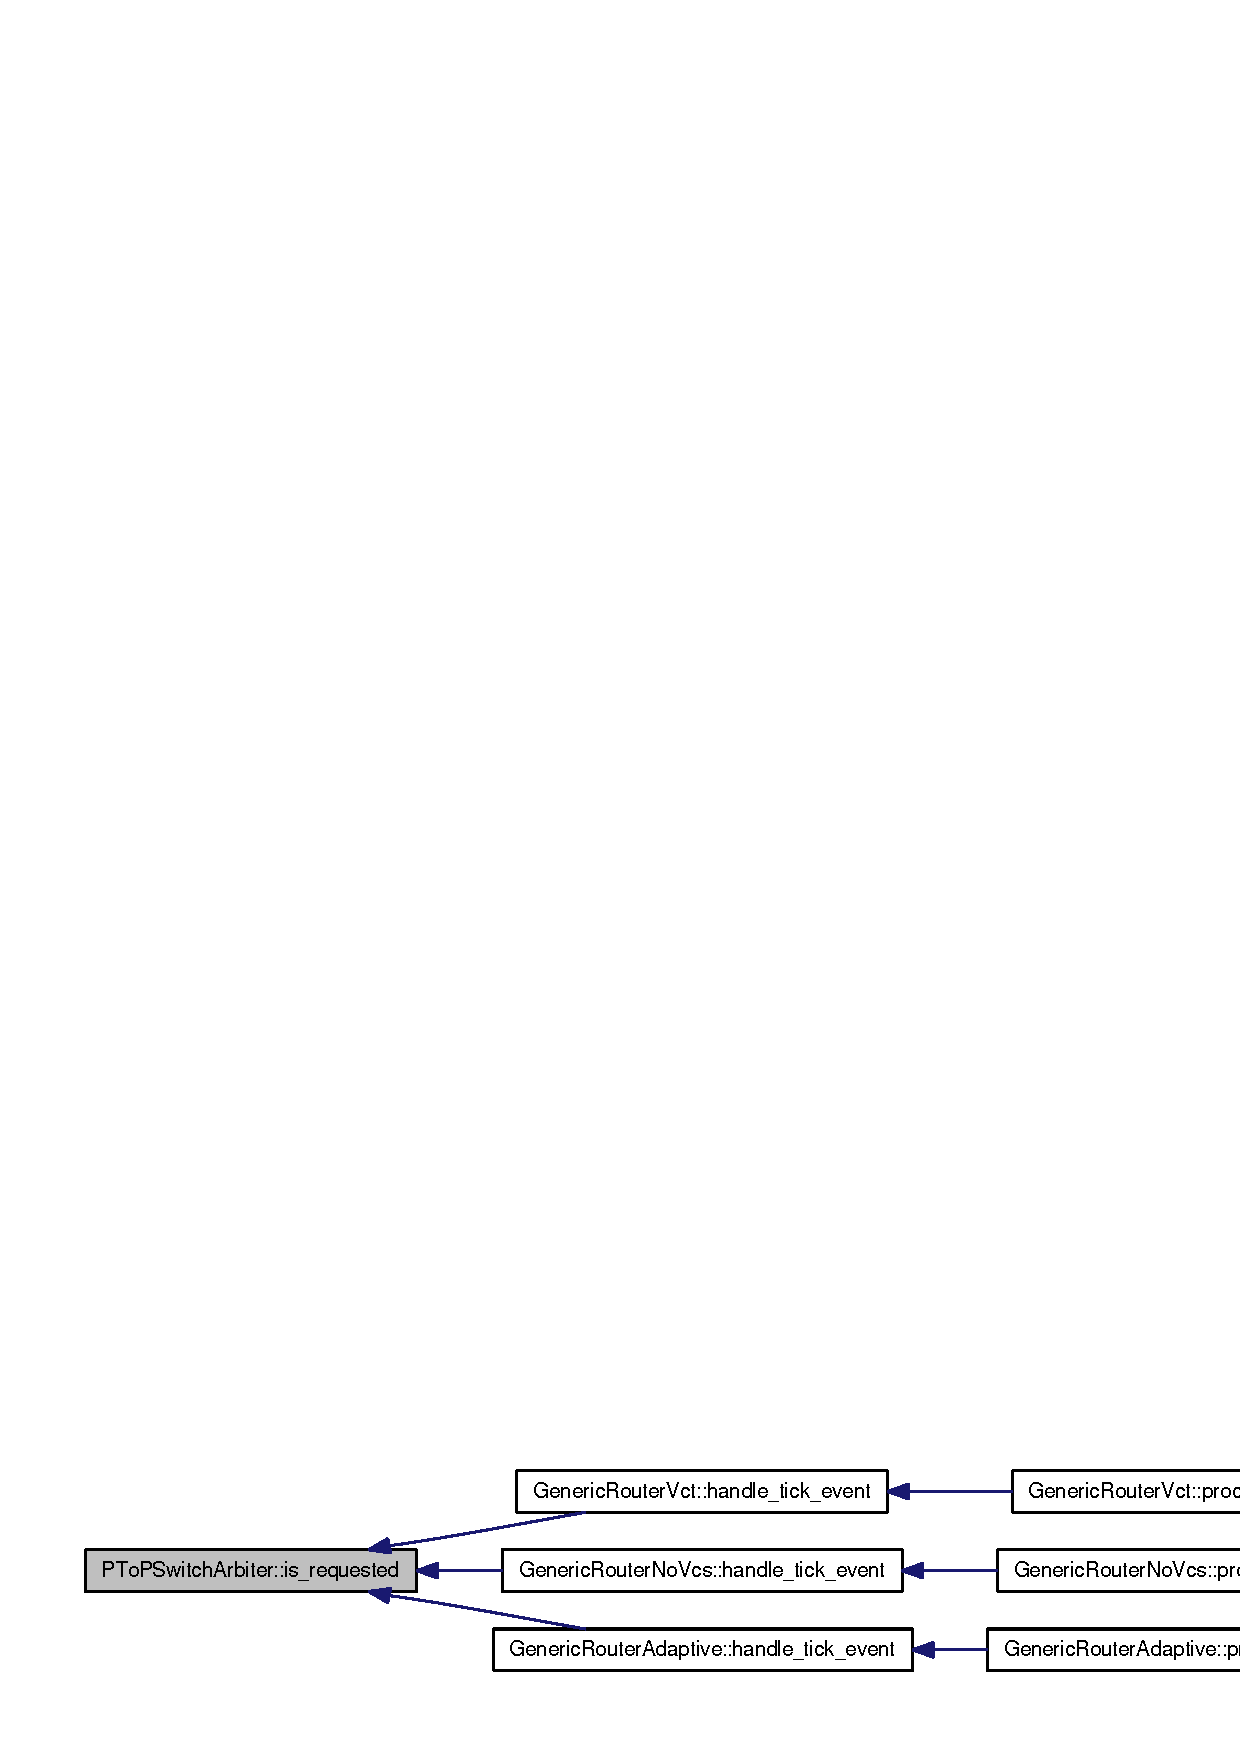
\includegraphics[width=332pt]{classPToPSwitchArbiter_3c4eeb723ecb521a82a4518820e48896_icgraph}
\end{center}
\end{figure}
\index{PToPSwitchArbiter@{PToPSwitchArbiter}!pick\_\-winner@{pick\_\-winner}}
\index{pick\_\-winner@{pick\_\-winner}!PToPSwitchArbiter@{PToPSwitchArbiter}}
\subsubsection[{pick\_\-winner}]{\setlength{\rightskip}{0pt plus 5cm}{\bf SA\_\-unit} PToPSwitchArbiter::pick\_\-winner ({\bf uint} {\em p})}\label{classPToPSwitchArbiter_8b304c2fc07b6c0d55ce25b621a9f685}




Definition at line 99 of file ptop\_\-swa.cc.

References do\_\-fcfs\_\-arbitration(), do\_\-priority\_\-round\_\-robin\_\-arbitration(), do\_\-round\_\-robin\_\-arbitration(), FCFS, ROUND\_\-ROBIN, ROUND\_\-ROBIN\_\-PRIORITY, and sw\_\-arbitration.

Referenced by GenericRouterVct::do\_\-switch\_\-allocation(), GenericRouterNoVcs::do\_\-switch\_\-allocation(), and GenericRouterAdaptive::do\_\-switch\_\-allocation().

Here is the caller graph for this function:\nopagebreak
\begin{figure}[H]
\begin{center}
\leavevmode
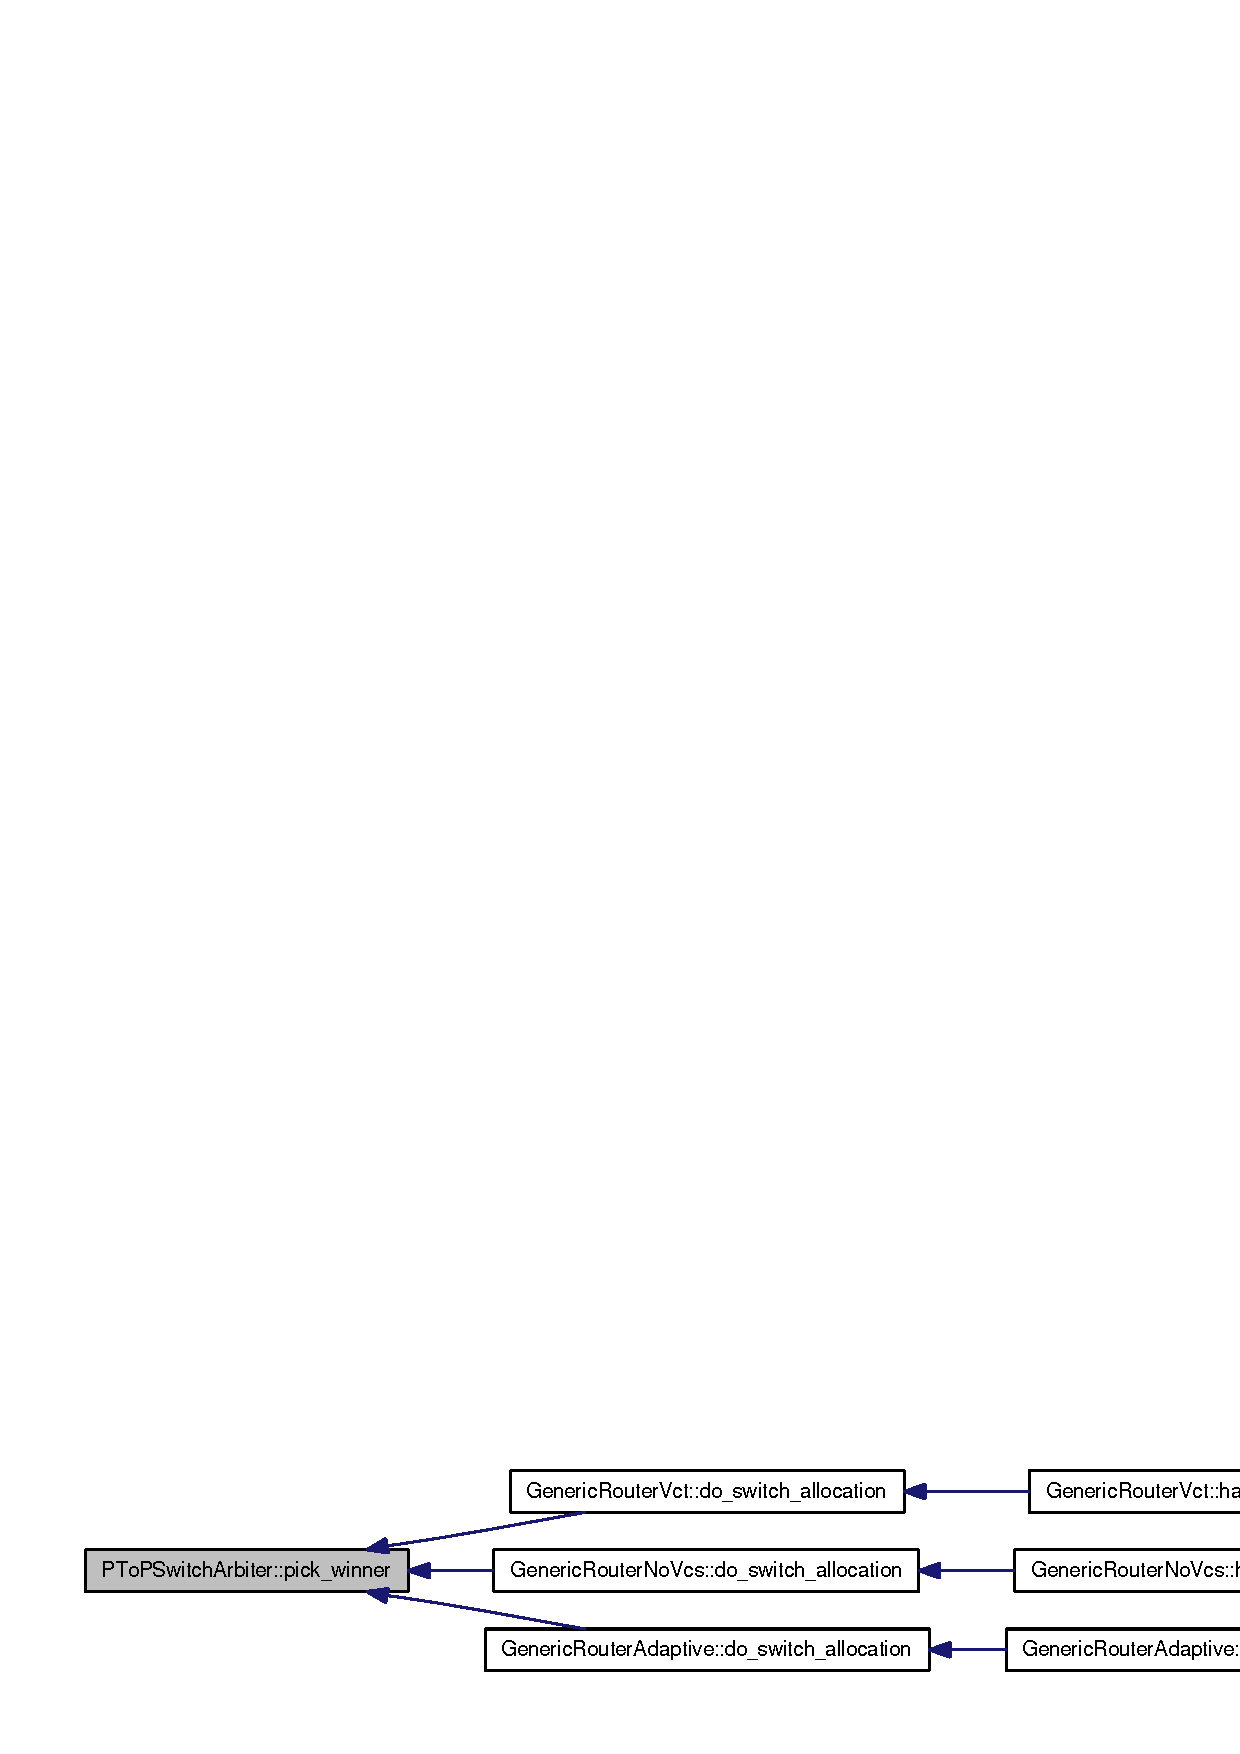
\includegraphics[width=420pt]{classPToPSwitchArbiter_8b304c2fc07b6c0d55ce25b621a9f685_icgraph}
\end{center}
\end{figure}
\index{PToPSwitchArbiter@{PToPSwitchArbiter}!request@{request}}
\index{request@{request}!PToPSwitchArbiter@{PToPSwitchArbiter}}
\subsubsection[{request}]{\setlength{\rightskip}{0pt plus 5cm}void PToPSwitchArbiter::request ({\bf uint} {\em oport}, \/  {\bf uint} {\em inport}, \/  {\bf message\_\-class} {\em m})}\label{classPToPSwitchArbiter_9cab6f94b19bb1ce2ec114d8570e5a07}




Definition at line 85 of file ptop\_\-swa.cc.

References done, Simulator::Now(), priority\_\-msg\_\-type, priority\_\-reqs, requested, and requesting\_\-inputs.\index{PToPSwitchArbiter@{PToPSwitchArbiter}!request@{request}}
\index{request@{request}!PToPSwitchArbiter@{PToPSwitchArbiter}}
\subsubsection[{request}]{\setlength{\rightskip}{0pt plus 5cm}void PToPSwitchArbiter::request ({\bf uint} {\em p}, \/  {\bf uint} {\em inp})}\label{classPToPSwitchArbiter_34e8394265869ee076610c67e4cf5de7}




Definition at line 75 of file ptop\_\-swa.cc.

References done, Simulator::Now(), requested, and requesting\_\-inputs.

Referenced by GenericRouterVct::handle\_\-tick\_\-event(), GenericRouterNoVcs::handle\_\-tick\_\-event(), and GenericRouterAdaptive::handle\_\-tick\_\-event().

Here is the caller graph for this function:\nopagebreak
\begin{figure}[H]
\begin{center}
\leavevmode
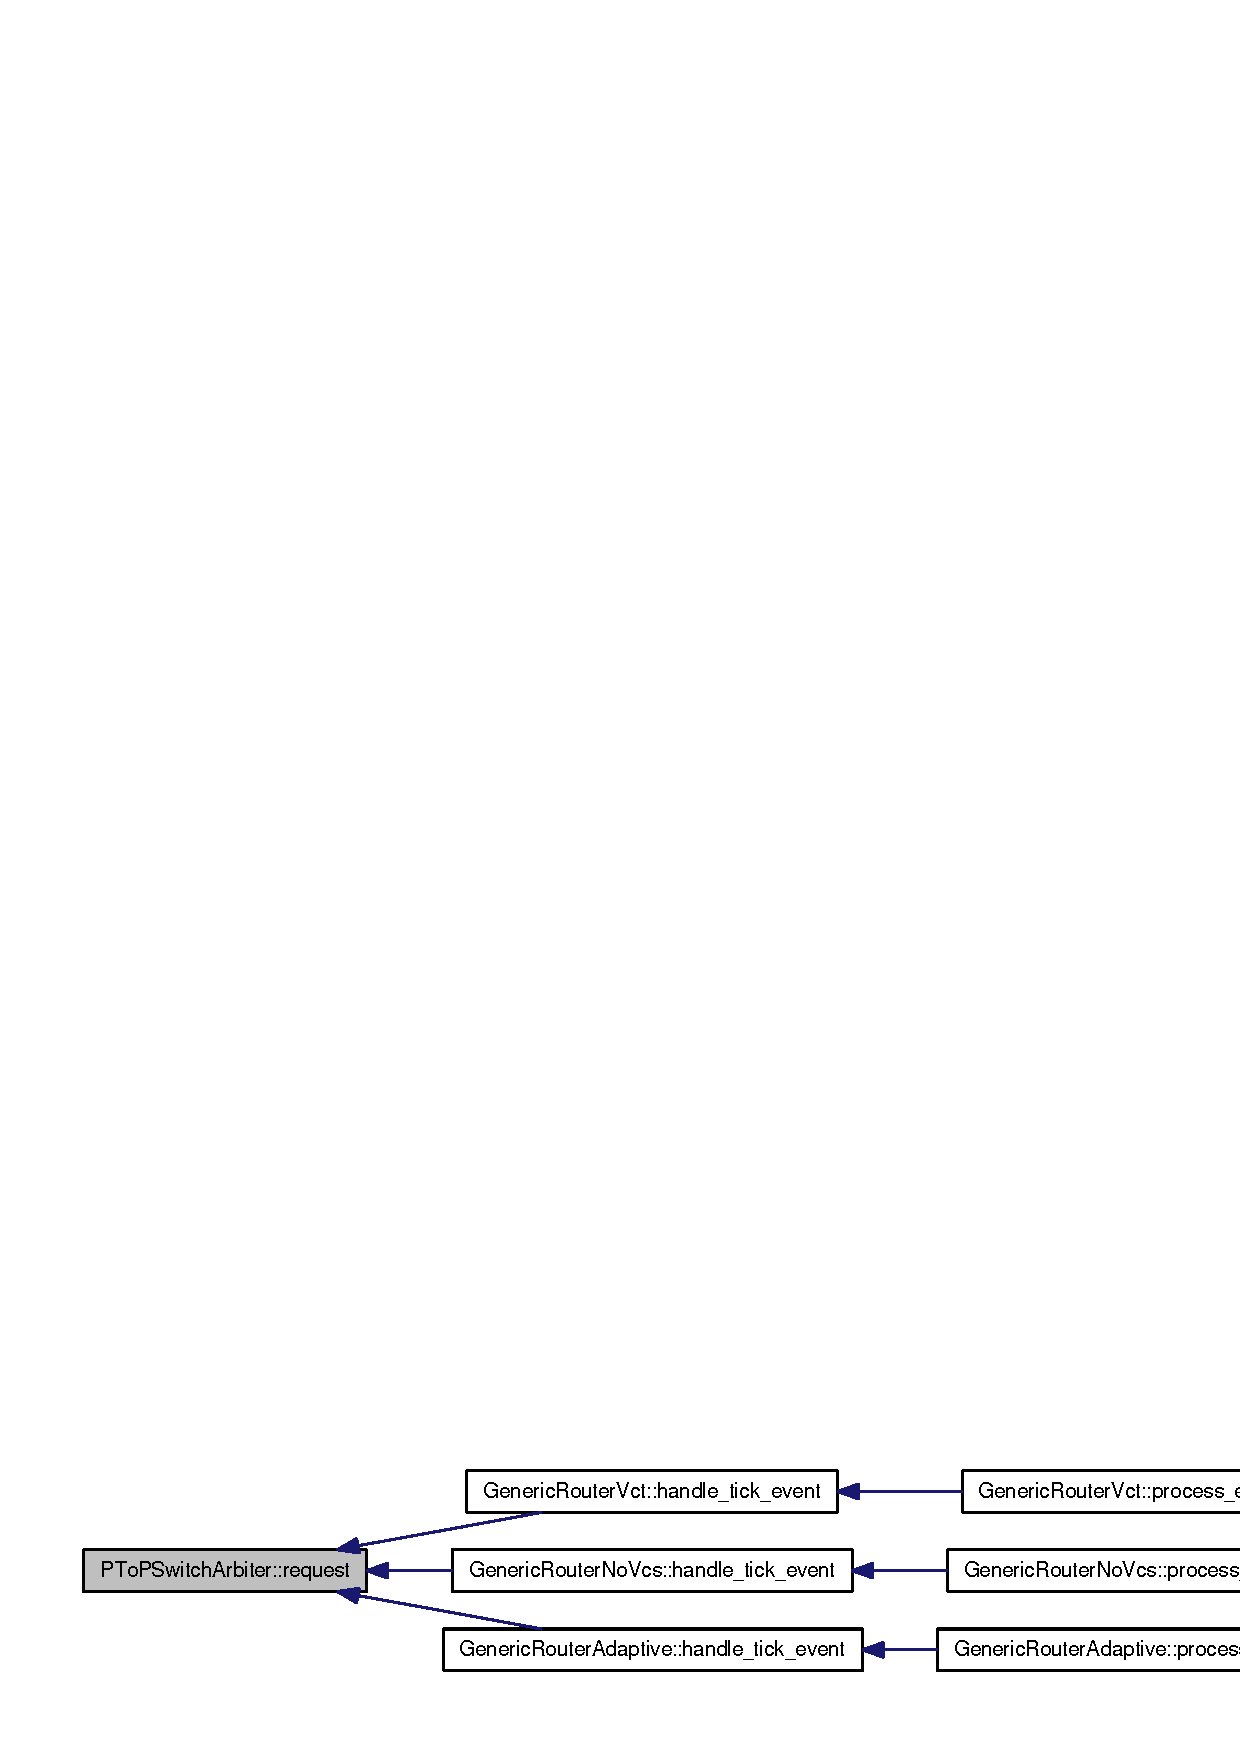
\includegraphics[width=320pt]{classPToPSwitchArbiter_34e8394265869ee076610c67e4cf5de7_icgraph}
\end{center}
\end{figure}
\index{PToPSwitchArbiter@{PToPSwitchArbiter}!resize@{resize}}
\index{resize@{resize}!PToPSwitchArbiter@{PToPSwitchArbiter}}
\subsubsection[{resize}]{\setlength{\rightskip}{0pt plus 5cm}void PToPSwitchArbiter::resize ({\bf uint} {\em p})}\label{classPToPSwitchArbiter_73fb7254a91aeeb209fa3225f09b1847}




Definition at line 34 of file ptop\_\-swa.cc.

References done, last\_\-port\_\-winner, last\_\-winner, locked, port\_\-locked, PORTS, priority\_\-reqs, requested, and requesting\_\-inputs.

Referenced by GenericRouterVct::init(), GenericRouterNoVcs::init(), and GenericRouterAdaptive::init().

Here is the caller graph for this function:\nopagebreak
\begin{figure}[H]
\begin{center}
\leavevmode
\includegraphics[width=173pt]{classPToPSwitchArbiter_73fb7254a91aeeb209fa3225f09b1847_icgraph}
\end{center}
\end{figure}
\index{PToPSwitchArbiter@{PToPSwitchArbiter}!toString@{toString}}
\index{toString@{toString}!PToPSwitchArbiter@{PToPSwitchArbiter}}
\subsubsection[{toString}]{\setlength{\rightskip}{0pt plus 5cm}string PToPSwitchArbiter::toString () const}\label{classPToPSwitchArbiter_f85a552b1be155e2717c197a51799414}




Definition at line 320 of file ptop\_\-swa.cc.

References requested.

Referenced by GenericRouterVct::toString(), GenericRouterNoVcs::toString(), and GenericRouterAdaptive::toString().

Here is the caller graph for this function:\nopagebreak
\begin{figure}[H]
\begin{center}
\leavevmode
\includegraphics[width=420pt]{classPToPSwitchArbiter_f85a552b1be155e2717c197a51799414_icgraph}
\end{center}
\end{figure}


\subsection{Member Data Documentation}
\index{PToPSwitchArbiter@{PToPSwitchArbiter}!address@{address}}
\index{address@{address}!PToPSwitchArbiter@{PToPSwitchArbiter}}
\subsubsection[{address}]{\setlength{\rightskip}{0pt plus 5cm}{\bf uint} {\bf PToPSwitchArbiter::address}}\label{classPToPSwitchArbiter_a01c0b9c63131ca029da5129d417ce0e}




Definition at line 47 of file ptop\_\-swa.h.

Referenced by GenericRouterAdaptive::init().\index{PToPSwitchArbiter@{PToPSwitchArbiter}!CHANNELS@{CHANNELS}}
\index{CHANNELS@{CHANNELS}!PToPSwitchArbiter@{PToPSwitchArbiter}}
\subsubsection[{CHANNELS}]{\setlength{\rightskip}{0pt plus 5cm}{\bf uint} {\bf PToPSwitchArbiter::CHANNELS}\hspace{0.3cm}{\tt  [private]}}\label{classPToPSwitchArbiter_7d44089feeffb503774491929479d17e}




Definition at line 55 of file ptop\_\-swa.h.\index{PToPSwitchArbiter@{PToPSwitchArbiter}!done@{done}}
\index{done@{done}!PToPSwitchArbiter@{PToPSwitchArbiter}}
\subsubsection[{done}]{\setlength{\rightskip}{0pt plus 5cm}vector$<$ bool$>$ {\bf PToPSwitchArbiter::done}\hspace{0.3cm}{\tt  [private]}}\label{classPToPSwitchArbiter_cbdde7ef64128ddefe4cd4ab9a145473}




Definition at line 57 of file ptop\_\-swa.h.

Referenced by clear\_\-winner(), do\_\-fcfs\_\-arbitration(), do\_\-priority\_\-round\_\-robin\_\-arbitration(), do\_\-round\_\-robin\_\-arbitration(), request(), and resize().\index{PToPSwitchArbiter@{PToPSwitchArbiter}!last\_\-port\_\-winner@{last\_\-port\_\-winner}}
\index{last\_\-port\_\-winner@{last\_\-port\_\-winner}!PToPSwitchArbiter@{PToPSwitchArbiter}}
\subsubsection[{last\_\-port\_\-winner}]{\setlength{\rightskip}{0pt plus 5cm}vector$<$ {\bf uint}$>$ {\bf PToPSwitchArbiter::last\_\-port\_\-winner}\hspace{0.3cm}{\tt  [private]}}\label{classPToPSwitchArbiter_734777a5e9b87a0785a0ebb6a0d1fb58}




Definition at line 63 of file ptop\_\-swa.h.

Referenced by do\_\-priority\_\-round\_\-robin\_\-arbitration(), do\_\-round\_\-robin\_\-arbitration(), and resize().\index{PToPSwitchArbiter@{PToPSwitchArbiter}!last\_\-winner@{last\_\-winner}}
\index{last\_\-winner@{last\_\-winner}!PToPSwitchArbiter@{PToPSwitchArbiter}}
\subsubsection[{last\_\-winner}]{\setlength{\rightskip}{0pt plus 5cm}vector$<$ {\bf SA\_\-unit} $>$ {\bf PToPSwitchArbiter::last\_\-winner}\hspace{0.3cm}{\tt  [private]}}\label{classPToPSwitchArbiter_5947d4082d52451d2e9838981dfc559d}




Definition at line 62 of file ptop\_\-swa.h.

Referenced by do\_\-fcfs\_\-arbitration(), do\_\-priority\_\-round\_\-robin\_\-arbitration(), do\_\-round\_\-robin\_\-arbitration(), and resize().\index{PToPSwitchArbiter@{PToPSwitchArbiter}!locked@{locked}}
\index{locked@{locked}!PToPSwitchArbiter@{PToPSwitchArbiter}}
\subsubsection[{locked}]{\setlength{\rightskip}{0pt plus 5cm}vector$<$ bool$>$ {\bf PToPSwitchArbiter::locked}\hspace{0.3cm}{\tt  [private]}}\label{classPToPSwitchArbiter_657970aaa9fab00ca0bb7d9e4ea80415}




Definition at line 56 of file ptop\_\-swa.h.

Referenced by clear\_\-winner(), do\_\-fcfs\_\-arbitration(), do\_\-priority\_\-round\_\-robin\_\-arbitration(), do\_\-round\_\-robin\_\-arbitration(), and resize().\index{PToPSwitchArbiter@{PToPSwitchArbiter}!name@{name}}
\index{name@{name}!PToPSwitchArbiter@{PToPSwitchArbiter}}
\subsubsection[{name}]{\setlength{\rightskip}{0pt plus 5cm}string {\bf PToPSwitchArbiter::name}}\label{classPToPSwitchArbiter_5b08d50980b7bde1801d19a57a223d00}




Definition at line 48 of file ptop\_\-swa.h.

Referenced by PToPSwitchArbiter().\index{PToPSwitchArbiter@{PToPSwitchArbiter}!node\_\-ip@{node\_\-ip}}
\index{node\_\-ip@{node\_\-ip}!PToPSwitchArbiter@{PToPSwitchArbiter}}
\subsubsection[{node\_\-ip}]{\setlength{\rightskip}{0pt plus 5cm}{\bf uint} {\bf PToPSwitchArbiter::node\_\-ip}}\label{classPToPSwitchArbiter_f6d6c3726dfca65b1dec2d041ce29e97}




Definition at line 49 of file ptop\_\-swa.h.

Referenced by GenericRouterAdaptive::init().\index{PToPSwitchArbiter@{PToPSwitchArbiter}!port\_\-locked@{port\_\-locked}}
\index{port\_\-locked@{port\_\-locked}!PToPSwitchArbiter@{PToPSwitchArbiter}}
\subsubsection[{port\_\-locked}]{\setlength{\rightskip}{0pt plus 5cm}vector$<$ bool$>$ {\bf PToPSwitchArbiter::port\_\-locked}\hspace{0.3cm}{\tt  [private]}}\label{classPToPSwitchArbiter_b512f01d5e4e47a1fee79144e66238aa}




Definition at line 60 of file ptop\_\-swa.h.

Referenced by resize().\index{PToPSwitchArbiter@{PToPSwitchArbiter}!PORTS@{PORTS}}
\index{PORTS@{PORTS}!PToPSwitchArbiter@{PToPSwitchArbiter}}
\subsubsection[{PORTS}]{\setlength{\rightskip}{0pt plus 5cm}{\bf uint} {\bf PToPSwitchArbiter::PORTS}\hspace{0.3cm}{\tt  [private]}}\label{classPToPSwitchArbiter_a3e7315bd5c36505d05e57f21306632e}




Definition at line 54 of file ptop\_\-swa.h.

Referenced by do\_\-fcfs\_\-arbitration(), do\_\-priority\_\-round\_\-robin\_\-arbitration(), do\_\-round\_\-robin\_\-arbitration(), is\_\-empty(), and resize().\index{PToPSwitchArbiter@{PToPSwitchArbiter}!priority\_\-reqs@{priority\_\-reqs}}
\index{priority\_\-reqs@{priority\_\-reqs}!PToPSwitchArbiter@{PToPSwitchArbiter}}
\subsubsection[{priority\_\-reqs}]{\setlength{\rightskip}{0pt plus 5cm}vector$<$ vector $<$bool$>$ $>$ {\bf PToPSwitchArbiter::priority\_\-reqs}\hspace{0.3cm}{\tt  [private]}}\label{classPToPSwitchArbiter_1d935ad033dbac73c9ef14fd279d0356}




Definition at line 59 of file ptop\_\-swa.h.

Referenced by clear\_\-requested(), clear\_\-winner(), do\_\-priority\_\-round\_\-robin\_\-arbitration(), request(), and resize().\index{PToPSwitchArbiter@{PToPSwitchArbiter}!requested@{requested}}
\index{requested@{requested}!PToPSwitchArbiter@{PToPSwitchArbiter}}
\subsubsection[{requested}]{\setlength{\rightskip}{0pt plus 5cm}vector$<$ vector $<$bool$>$ $>$ {\bf PToPSwitchArbiter::requested}\hspace{0.3cm}{\tt  [private]}}\label{classPToPSwitchArbiter_191d12127b578016fc532f2fc00677c2}




Definition at line 58 of file ptop\_\-swa.h.

Referenced by clear\_\-requested(), clear\_\-winner(), do\_\-fcfs\_\-arbitration(), do\_\-priority\_\-round\_\-robin\_\-arbitration(), do\_\-round\_\-robin\_\-arbitration(), is\_\-empty(), is\_\-requested(), request(), resize(), and toString().\index{PToPSwitchArbiter@{PToPSwitchArbiter}!requesting\_\-inputs@{requesting\_\-inputs}}
\index{requesting\_\-inputs@{requesting\_\-inputs}!PToPSwitchArbiter@{PToPSwitchArbiter}}
\subsubsection[{requesting\_\-inputs}]{\setlength{\rightskip}{0pt plus 5cm}vector$<$ vector$<${\bf SA\_\-unit}$>$ $>$ {\bf PToPSwitchArbiter::requesting\_\-inputs}\hspace{0.3cm}{\tt  [private]}}\label{classPToPSwitchArbiter_56dde672e0b26a80ee6a9491695bfa75}




Definition at line 61 of file ptop\_\-swa.h.

Referenced by do\_\-fcfs\_\-arbitration(), do\_\-priority\_\-round\_\-robin\_\-arbitration(), do\_\-round\_\-robin\_\-arbitration(), request(), and resize().

The documentation for this class was generated from the following files:\begin{CompactItemize}
\item 
{\bf ptop\_\-swa.h}\item 
{\bf ptop\_\-swa.cc}\end{CompactItemize}
